%!Mode:: "TeX:UTF-8"
\documentclass[a4paper,11pt,UTF8]{ctexart}
\usepackage{indentfirst} %缩进
\usepackage{xeCJK}    %使用系统字体
\usepackage{fancyhdr} %自定义页眉页脚
\pagestyle{empty}                   %不设置页眉页脚
\usepackage{amsmath, amsthm, amssymb, amsfonts} %数学公式
\usepackage[a4paper,left=3cm,right=3cm,top=3cm,bottom=3cm]{geometry}
%\usepackage[tmargin=1in,bmargin=1in,lmargin=1.25in,rmargin=1.25in]{geometry}.
\usepackage{booktabs} %插入表格
\usepackage[section]{placeins} %避免浮动
\usepackage{listings} %插入代码
\usepackage{ctex}     %中文宏包
\usepackage[svgnames, table]{xcolor} %彩色表格
\usepackage{algorithm}          %伪代码
\usepackage{algorithmicx}
\usepackage{algpseudocode}
\usepackage{algorithm,algpseudocode,float}
\usepackage{lipsum}
\usepackage{enumitem}           %调整列举环境
\usepackage{url}
\usepackage{fontspec,xunicode}
\usepackage{cite}
\defaultfontfeatures{Mapping=tex-text} %如果没有它,会有一些 tex 特殊字符无法正常使用,比如连字符。

\usepackage{graphicx}
\usepackage{subfigure}
\graphicspath{{imgs/}}

%%%%%%%%%%%%%%%%%%%%%%%%%%%%%%%%%%%%%%%%%%%%%%%%%%%%%%%%%%%%%%%%
% 缩进及行间距
%%%%%%%%%%%%%%%%%%%%%%%%%%%%%%%%%%%%%%%%%%%%%%%%%%%%%%%%%%%%%%%%
\setlength{\parindent}{22pt} %重新定义缩进长度
\setlength{\baselineskip}{20pt}  %定义行间距
%\renewcommand{\baselinestretch}{1.1} %定义行间距

%%%%%%%%%%%%%%%%%%%%%%%%%%%%%%%%%%%%%%%%%%%%%%%%%%%%%%%%%%%%%%%%
% 列表设置
%%%%%%%%%%%%%%%%%%%%%%%%%%%%%%%%%%%%%%%%%%%%%%%%%%%%%%%%%%%%%%%%
\setenumerate{fullwidth,itemindent=\parindent,listparindent=\parindent,itemsep=0ex,partopsep=0pt,parsep=0ex}
\setenumerate[2]{label=\alph*),leftmargin=1.5em}  %二级item设置
\setitemize{itemindent=38pt,leftmargin=0pt,itemsep=-0.4ex,listparindent=26pt,partopsep=0pt,parsep=0.5ex,topsep=-0.25ex}
\setdescription{itemindent=38pt,leftmargin=0pt,itemsep=-0.4ex,listparindent=26pt,partopsep=0pt,parsep=0.5ex,topsep=-0.25ex}

%%%%%%%%%%%%%%%%%%%%%%%%%%%%%%%%%%%%%%%%%%%%%%%%%%%%%%%%%%%%%%%%
% 图的标题行间距设置
%%%%%%%%%%%%%%%%%%%%%%%%%%%%%%%%%%%%%%%%%%%%%%%%%%%%%%%%%%%%%%%%
\newcommand{\bottomcaption}{%
\setlength{\abovecaptionskip}{6pt}%
\setlength{\belowcaptionskip}{6pt}%
\caption}


%%%%%%%%%%%%%%%%%%%%%%%%%%%%%%%%%%%%%%%%%%%%%%%%%%%%%%%%%%%%%%%%
% 字体定义
%%%%%%%%%%%%%%%%%%%%%%%%%%%%%%%%%%%%%%%%%%%%%%%%%%%%%%%%%%%%%%%%
\setmainfont{Times New Roman}  %默认英文字体.serif是有衬线字体sans serif无衬线字体
\setmonofont{Consolas}
\setCJKmainfont[ItalicFont={楷体}, BoldFont={黑体}]{宋体}%衬线字体 缺省中文字体为
\setCJKsansfont{黑体}
\punctstyle{hangmobanjiao}
%-----------------------xeCJK下设置中文字体------------------------------%
\setCJKfamilyfont{song}{SimSun}                             %宋体 song
\newcommand{\song}{\CJKfamily{song}}
\setCJKfamilyfont{fs}{FangSong}                      %仿宋  fs
\newcommand{\fs}{\CJKfamily{fs}}
\setCJKfamilyfont{ktgb}{KaiTi}                      %楷体2312 ktgb
\newcommand{\ktgb}{\CJKfamily{ktgb}}
\setCJKfamilyfont{yh}{Microsoft YaHei}                    %微软雅黑 yh
\newcommand{\yh}{\CJKfamily{yh}}
\setCJKfamilyfont{hei}{SimHei}                              %黑体  hei
\newcommand{\hei}{\CJKfamily{hei}}
\setCJKfamilyfont{hwxk}{STXingkai}                                %华文行楷  hwxk
\newcommand{\hwxk}{\CJKfamily{hwxk}}
%------------------------------设置字体大小------------------------%
\newcommand{\shiyanbaogao}{\fontsize{36pt}{\baselineskip}\selectfont}
\newcommand{\chuhao}{\fontsize{42pt}{\baselineskip}\selectfont}     %初号
\newcommand{\xiaochuhao}{\fontsize{36pt}{\baselineskip}\selectfont} %小初号
\newcommand{\yihao}{\fontsize{28pt}{\baselineskip}\selectfont}      %一号
\newcommand{\erhao}{\fontsize{21pt}{\baselineskip}\selectfont}      %二号
\newcommand{\xiaoerhao}{\fontsize{18pt}{\baselineskip}\selectfont}  %小二号
\newcommand{\sanhao}{\fontsize{15.75pt}{\baselineskip}\selectfont}  %三号
\newcommand{\sihao}{\fontsize{14pt}{\baselineskip}\selectfont}       %四号
\newcommand{\xiaosihao}{\fontsize{12pt}{\baselineskip}\selectfont}  %小四号
\newcommand{\wuhao}{\fontsize{10.5pt}{\baselineskip}\selectfont}    %五号
\newcommand{\xiaowuhao}{\fontsize{9pt}{\baselineskip}\selectfont}   %小五号
\newcommand{\liuhao}{\fontsize{7.875pt}{\baselineskip}\selectfont}  %六号
\newcommand{\qihao}{\fontsize{5.25pt}{\baselineskip}\selectfont}    %七号

%%%%%%%%%%%%%%%%%%%%%%%%%%%%%%%%%%%%%%%%%%%%%%%%%%%%%%%%%%%%%%%%
% 图题字体大小相同
%%%%%%%%%%%%%%%%%%%%%%%%%%%%%%%%%%%%%%%%%%%%%%%%%%%%%%%%%%%%%%%%
\usepackage{caption}
\captionsetup{font={footnotesize}}   % footnotesize = 9pt
\captionsetup[lstlisting]{font={footnotesize}}

%%%%%%%%%%%%%%%%%%%%%%%%%%%%%%%%%%%%%%%%%%%%%%%%%%%%%%%%%%%%%%%%
% 重定义枚举编号为 1),2)...
%%%%%%%%%%%%%%%%%%%%%%%%%%%%%%%%%%%%%%%%%%%%%%%%%%%%%%%%%%%%%%%%
\renewcommand{\labelenumi}{\theenumi)}


%%%%%%%%%%%%%%%%%%%%%%%%%%%%%%%%%%%%%%%%%%%%%%%%%%%%%%%%%%%%%%%%
% 重定义section标题
%%%%%%%%%%%%%%%%%%%%%%%%%%%%%%%%%%%%%%%%%%%%%%%%%%%%%%%%%%%%%%%%
\CTEXsetup[format={\sihao\CJKfamily{zhhei}\zihao{4}},number={\chinese{section}},name={,、~},aftername={},indent={0pt},beforeskip={6pt},afterskip={6pt},format+={\flushleft}]{section}
\CTEXsetup[format={\Large\bfseries\CJKfamily{zhkai}\zihao{5}},name={(,)},number={\chinese{subsection}},aftername={},indent={22pt},beforeskip={14pt},afterskip={2pt}]{subsection}
\CTEXsetup[number={\chinese{section}},name={附录, ~~ }]{appendix}



%%%%%%%%%%%%%%%%%%%%%%%%%%%%%%%%%%%%%%%%%%%%%%%%%%%%%%%%%%%%%%%%
% 标题名称中文化
%%%%%%%%%%%%%%%%%%%%%%%%%%%%%%%%%%%%%%%%%%%%%%%%%%%%%%%%%%%%%%%%
\renewcommand\figurename{\hei 图}
\renewcommand\tablename{\hei 表}
\renewcommand\lstlistingname{\hei 代码}
\renewcommand{\algorithmicrequire}{\textbf{输入:}}
\renewcommand{\algorithmicensure}{\textbf{输出:}}
\newtheorem{define}{定义}

%%%%%%%%%%%%%%%%%%%%%%%%%%%%%%%%%%%%%%%%%%%%%%%%%%%%%%%%%%%%%%%%
% 代码设置
%%%%%%%%%%%%%%%%%%%%%%%%%%%%%%%%%%%%%%%%%%%%%%%%%%%%%%%%%%%%%%%%
\lstset{
 columns=fixed,
 numbers=left,                                        % 在左侧显示行号
 numberstyle=\tiny\color{gray},                       % 设定行号格式
 frame=single,                                        % 单线背景边框
 breaklines=true,                                     % 设定LaTeX对过长的代码行进行自动换行
 keywordstyle=\color[RGB]{40,40,255},                 % 设定关键字颜色
 numberstyle=\footnotesize\color{darkgray},
 commentstyle=\it\color[RGB]{0,96,96},                % 设置代码注释的格式
 stringstyle=\rmfamily\slshape\color[RGB]{128,0,0},   % 设置字符串格式
 showstringspaces=false,                              % 不显示字符串中的空格
 language=java,                                        % 设置语言
 basicstyle=\linespread{1.0}\xiaowuhao\ttfamily,                      % 字体字号
 %lineskip=10pt,
 %baselinestretch=1,
}

%%%%%%%%%%%%%%%%%%%%%%%%%%%%%%%%%%%%%%%%%%%%%%%%%%%%%%%%%%%%%%%%
% 伪代码分页
%%%%%%%%%%%%%%%%%%%%%%%%%%%%%%%%%%%%%%%%%%%%%%%%%%%%%%%%%%%%%%%%
\makeatletter
\renewcommand{\ALG@name}{算法}
\newenvironment{breakablealgorithm}
  {% \begin{breakablealgorithm}
   \begin{center}
     \refstepcounter{algorithm}% New algorithm
     \hrule height.8pt depth0pt \kern2pt% \@fs@pre for \@fs@ruled
     \renewcommand{\caption}[2][\relax]{% Make a new \caption
       {\raggedright\textbf{\ALG@name~\thealgorithm} ##2\par}%
       \ifx\relax##1\relax % #1 is \relax
         \addcontentsline{loa}{algorithm}{\protect\numberline{\thealgorithm}##2}%
       \else % #1 is not \relax
         \addcontentsline{loa}{algorithm}{\protect\numberline{\thealgorithm}##1}%
       \fi
       \kern2pt\hrule\kern2pt
     }
  }{% \end{breakablealgorithm}
     \kern2pt\hrule\relax% \@fs@post for \@fs@ruled
   \end{center}
  }
\makeatother



\begin{document}
\xiaosihao\song

\begin{titlepage}
\center{\yihao{\ktgb{中山大学数据科学与计算机学院\\操作系统实验课程}}}
\vspace{1cm}


\center{\shiyanbaogao{\ktgb{实~验~报~告}}}
\vspace{2cm}

\begin{center}
\begin{large}
\begin{tabular}{rc}
\xiaoerhao{\hei{教\qquad 师}}& \sanhao{\hei{凌应标}}\\
\cline{2-2}\\
\xiaoerhao{\hei{学\qquad 号}}& \hspace{1.7cm}\sanhao{\hei{17341035\hspace{1.7cm}}} \\
\cline{2-2}\\
\xiaoerhao{\hei{姓\qquad 名}}& \sanhao{\hei{傅畅}}\\
\cline{2-2}\\
\xiaoerhao{\hei{实验名称}}& \sanhao{\hei{实验一(接管裸机控制权)}}\\
\cline{2-2}\\

\end{tabular}
\end{large}
\end{center}
\vfill \hfill
\end{titlepage}
\clearpage

\centerline{\\[10pt]\erhao{\fs{实~验~一}}}
\centerline{\\[10pt]\yihao{\fs{接~管~裸~机~控~制~权}}}

\leftline{\\[8pt]\xiaosihao{\hei{\hspace{1.5em} 姓名:傅畅\hfill 学号:17341038 \hfill  }}}

\leftline{\\[8pt]\xiaosihao{\hei{\hspace{1.5em} 邮箱:fuch8@mail2.sysu.edu.cn \hfill}}}

\leftline{\\[8pt]\xiaosihao{\hei{\hspace{1.5em} 实验时间:周五(3-4节) \hfill }}}


\setcounter{tocdepth}{2}
\setlength{\parskip}{0pt}
\tableofcontents
\clearpage

\section{实验目的}
	
	\begin{enumerate}
		\item 理解操作系统的定义、功能与作用,了解嵌入式开发基本原理。
		\item 掌握实验环境的构成与实验工具搭配,实现实验环境的搭建与简单应用。
		\item 掌握裸机编程基本操作流程,着重理解内存与地址空间,显存原理,寄存器使用规则,实现接管裸机的控制权。
	\end{enumerate}


\section{实验要求}

\subsection{搭建和应用实验环境}

	虚拟机安装,生成一个基本配置的虚拟机XXXPC和多个1.44MB容量的虚拟软盘,将其中一个虚拟软盘用DOS格式化为DOS引导盘,用WinHex工具将其中一个虚拟软盘的首扇区填满你的个人信息。
	

\subsection{接管裸机控制权}
	
    设计IBM\_PC的一个引导扇区程序,程序功能是:用字符‘A’从屏幕左边某行位置45度角下斜射出,保持一个可观察的适当速度直线运动,碰到屏幕的边后产生反射,改变方向运动,如此类推,不断运动;在此基础上,增加你的个性扩展,如同时控制两个运动的轨迹,或炫酷动态变色,个性画面,如此等等,自由不限。还要在屏幕某个区域特别的方式显示你的学号姓名等个人信息。将这个程序的机器码放进放进第三张虚拟软盘的首扇区,并用此软盘引导你的XXXPC,直到成功。
	

\section{实验方案}


\subsection{配置方法及相关工具说明}

\subsubsection{实验支撑环境}
	\begin{itemize} 
		\item 硬件:个人计算机
		\item 主机操作系统:Linux 4.18.0-16-generic 17-Ubuntu
		\item 虚拟机软件: Bochs 2.6.9
	\end{itemize}
	
	
	本次实验的程序开发工作在Linux环境下进行,便于调试与优化;存储与CPU等硬件资源来自PC,由虚拟机软件的调度算法控制。
	
	虚拟机为操作系统的运行提供一个虚拟化平台,它与主机的空间分离,理论上不会对主机的运行造成影响。即使实验操作系统崩溃,也可以通过重启虚拟机的方式继续实验。
	
	Bochs的使用依赖配置文件,通过配置文件指定不同的硬件,以及指定存储介质的映像文件(BIOS的ROM文件、磁盘文件等)。
	
	 
\subsubsection{实验开发工具}

	\begin{itemize} 
	\item 汇编语言工具: x86汇编
	\item 程序编辑器: VScode 
	\item x86汇编器: NASM\_v2.07
	\item 磁盘映像文件浏览编辑工具: wxHexEditor 0.23 Beta For Linux
	
	本次实验主要在VScode编辑平台上使用汇编语言模式完成。汇编程序使用NASM的汇编命令生成bin文件,然后使用wxHexEditor 检查格式完整,完成引导盘的设计。
\end{itemize}

\subsection{方案思想与程序流程}

	\begin{itemize}
	\item 多小球独立并发移动

	\item 程序设计
	
	程序的数据区主要包括小球个数n,每个小球的方向dir以及四个方向移动,所对应的坐标改变连量delx[4], dely[4]。
	同时另外开四个$db$变量:$counti, countj, countk ,countl$,用于下面程序实现循环时的计数
	
	程序在Initial 段完成段寄存器的赋值后,开始进入$show\rightarrow slide \rightarrow show$ 的循环,show的部分,是将n个小球的位置逐个打印到其(posx, posy)所对应的位置上;然后利用冗余循环等待若干ms之后,将原来被打印的位置清零,不保留上次移动的痕迹。slide的部分就是根据小球当前位置调整其下一步移动的方向,然后移动一步,并更新其位置。
	
	
	
	
\end{itemize}
	
\subsection{数据结构与算法}

	\begin{itemize}
		\item 数据结构: 数组
		
		使用若干个长度为n的数组,其中小球的坐标(x,y),运动方向($\delta x$, $\delta y$)使用了4个db数组, 转化后小球在屏幕上位置$(x*80+y)\times 2)$ 使用了一个dw数组。这样提升了代码的复用性与编程效率。
			
			
			\clearpage
			\lstset{language=={[x86masm]Assembler}}
			\begin{lstlisting}[caption={stone\_v0.asm数组定义},basicstyle=\footnotesize,tabsize=4,captionpos=b]
delx db 0x01,0x01,0xff,0xff
dely db 0x01,0xff,0x01,0xff  ; 00 01 10 11
posx db 0x00
posy db 0x00
poss dw 0x00
dir db 0x00

counti dw 0
countj dw 0
countk dw 0
countl dw 0
			\end{lstlisting}
			
		\item 算法: 循环模拟
		
		小球运动比较简单,直接模拟即可
		
	\end{itemize}

\subsection{程序关键模块说明}
	\begin{itemize}
		\item sleep
		
		sleep段主要完成延时与循环变量的清零。
			\lstset{language=={[x86nasm]Assembler}}
			\begin{lstlisting}[caption={stone.asm sleeploop段},tabsize=4,basicstyle=\footnotesize,captionpos=b]
	mov word[counti],delay
	mov word[countj],delay
sleeploop:
	dec word[counti]
	jnz sleeploop
	mov word[counti], delay
	dec word[countj]
	jnz sleeploop

			\end{lstlisting}

	
		\item loop1
		
		在前面已说明,此处仅贴代码。
		\lstset{language=={[x86nasm]Assembler}}
		\begin{lstlisting}[caption={stone\_v0.asm loop1段}, basicstyle=\footnotesize,tabsize=4,captionpos=b]
l	mov word [counti], posx
	mov word [countj], posy
	mov word [countk], n
	mov word [countl], poss
	loop1:
		mov ax, 0x0
		mov bx, 0x0
		mov dx, 0x0
		mov bx, [counti]  ; 取出循环变量i所指posx位置的值

		mov al, [bx]

		mov cx, 0x50  ;将x乘上行长度
		mul cx

		mov bx, [countj]  ;取出循环变量j所指posy位置的值
		mov dl, [bx]
		add ax,dx
		mov cx, 0x2
		mul cx

		mov bx, ax
		mov byte [es:bx],'*'
		mov byte [es:bx+0x01],0x07
		mov bx, [countl]  ;屏幕对应的实际位置,需要*2
		mov [bx], ax

		inc word [counti]
		inc word [countj]
		inc word [countl] ;循环变量l所指的poss是dw类型的变量,位长2Byte,所以每次循环要+2
		inc word [countl]
		dec word [countk]
	jnz loop1

		\end{lstlisting}
	
	\item Slide
	
	首先根据当前位置改变运动方向,然后移动位置
	
	\lstset{language=={[x86nasm]Assembler}}
	\begin{lstlisting}[caption={stone.asm slide段},tabsize=4,basicstyle=\footnotesize,captionpos=b]
slide:
	mov word [counti], posx
	mov word [countj], posy
	mov word [countl], dir
	mov word [countk], n
	loop3: 				;循化n次,对每个位置独立考虑
		mov bx,[counti]
		mov dl, [bx]
		mov bx,[countj]  ;取出x,y坐标,分别放在dl,dh中
		mov dh, [bx]

		mov bx, [countl]
		mov al, [bx] 
		mov bx,0
		mov bl, al		;取出当前方向,放入bl
		mov al, [delx+bx]  ;将$\Delta x \Delta y$分别放入al, ah
		mov ah, [dely+bx]

		add dl,al      ;计算沿当前方向运动到的目标位置
		add dh,ah

		mov cl, bl
		cmp dl, 0xff    
		jne Endjudge1   
			xor cl,0x02  ;如果dl<0,改变$\Delta x$的方向
 			mov bx,[countl]
			mov [bx],cl
			jmp near loop3
		Endjudge1:

		cmp dl, LimitX  ;如果dl>LimitX,改变$\Delta x$的方向
		jne Endjudge2
			xor cl,0x2
			mov bx,[countl]
			mov [bx],cl
			jmp near loop3
		Endjudge2:

		cmp dh, 0xff 			 ;如果dh<0,改变$\Delta y$的方向
		jne Endjudge3
			xor cl,0x01
			mov bx,[countl]
			mov [bx],cl
			jmp near loop3
		Endjudge3:

		cmp dh,LimitY		 ;如果dh>=LimitY,改变$\Delta y$的方向
		jne Endjudge4
			xor cl, 0x01
			mov bx,[countl]
			mov [bx],cl
			jmp near loop3
		Endjudge4:
		
		mov bx, [countl] 			;将新的坐标和方向从寄存器中放回主存
		mov [bx],cl
		mov bx, [counti]
		mov [bx], dl
		mov bx, [countj]
		mov [bx], dh

		inc word[counti]
		inc word [countj]
		inc word [countl]
		dec word [countk]
	jnz loop3

jmp near show
	
	\end{lstlisting}
	

	

	
	\end{itemize}


\section{实验过程与结果}

\subsection{工具安装及使用}

这一部分主要解决要求1。
\subsubsection{工具安装}

	\begin{itemize}
		\item bochs 虚拟机安装时直接按照网络教程执行,没有什么大的烦恼
		
		\item NASM
		
		Linux下安装直接sudo apt-get install nasm即可
	
		\item wxHexEditor 0.32 Beta for Linux
		
		在ubuntu下直接sudo apt-get install wxhexeditor	
	\end{itemize}

\subsubsection{工具使用}

	\begin{enumerate}
		\item 配置bochs的指定映像文件
		
\lstset{language=={[x86nasm]Assembler}}
	\begin{lstlisting}[caption={bochsrc},tabsize=4,basicstyle=\footnotesize,captionpos=b]
megs:128

romimage:file=/usr/local/share/bochs/gdb/share/bochs/BIOS-bochs-latest
vgaromimage:file=/usr/local/share/bochs/gdb/share/bochs/VGABIOS-lgpl-latest

floppya:1\_44=vfdd144,status=inserted
boot:floppy

log:bochsout.txt

mouse:enabled=0

display_library:x, options="gui_debug"

#gdbstub: enabled=1, port=1234, text_base=0, data_base=0, bss_base=0
	\end{lstlisting}
	
	
		
		
	\end{enumerate}
\subsection{实验操作说明与程序运行结果}
	这一部分主要用于解决要求2。首先使用NASM的汇编命令:nasm -f bin stone\_v0.asm -o vfdd144

	\begin{figure}[htbp]
		\centering
		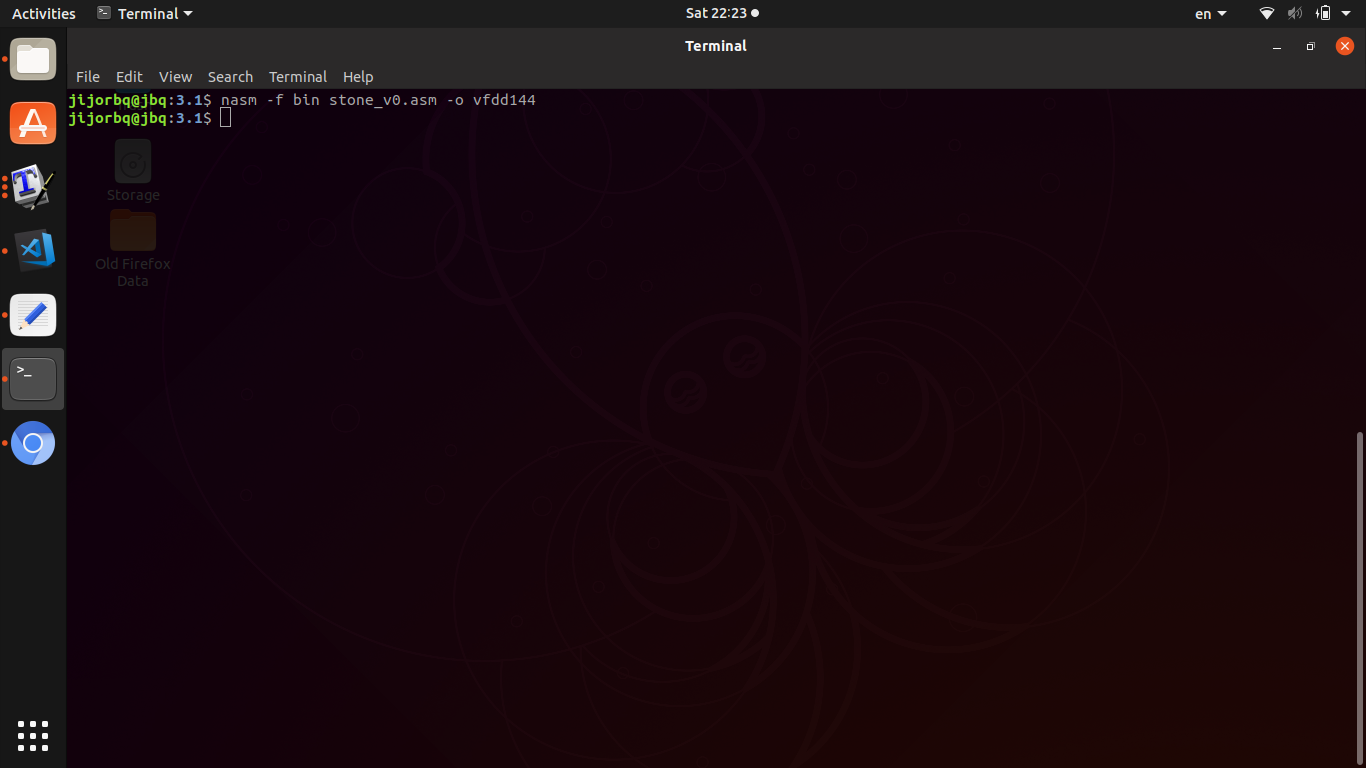
\includegraphics[width=10cm]{Screenshot from 2019-03-23 22-23-16.png}
		\bottomcaption{终端直接执行}
	\end{figure}
	终端直接执行:bochs -q -f bochsrc

	\begin{figure}[htbp]
		\centering
		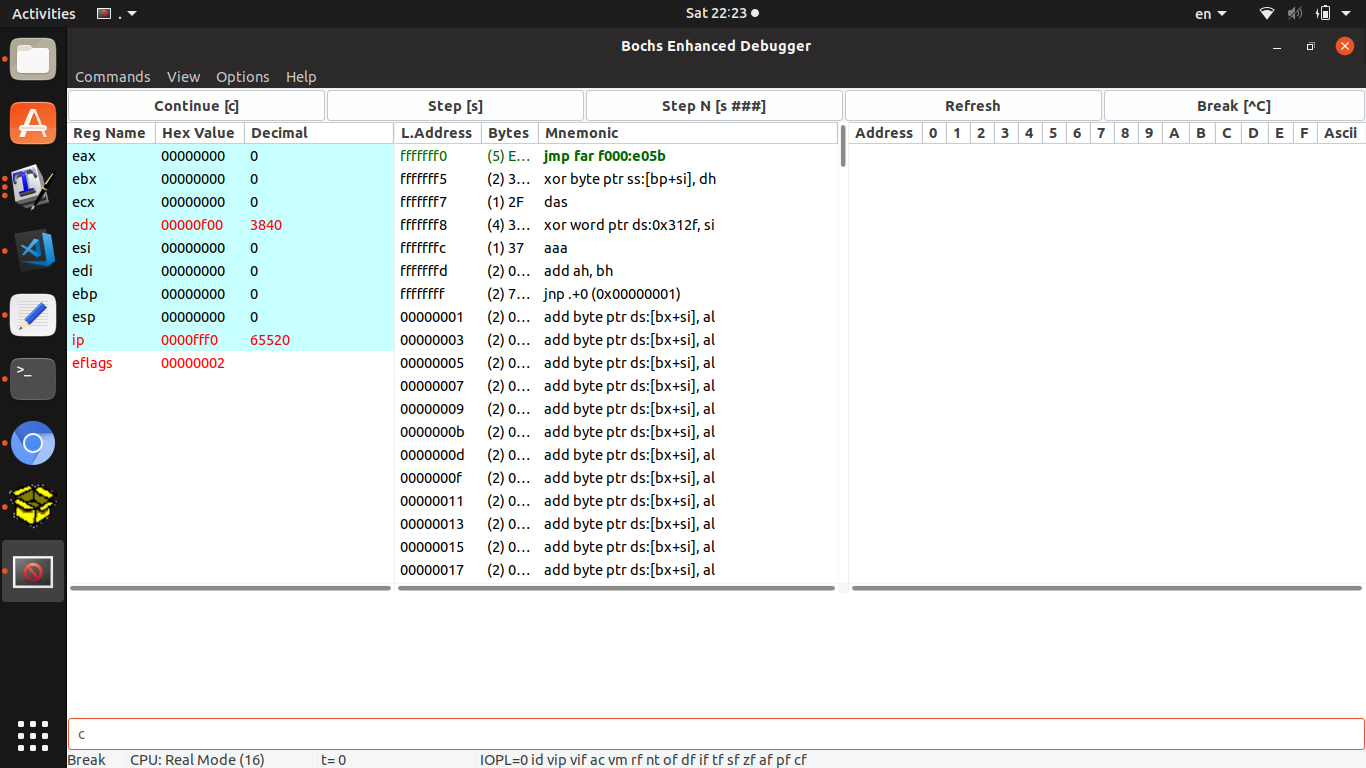
\includegraphics[width=10cm]{Screenshot from 2019-03-23 22-23-35.png}
		\bottomcaption{打开bochs}
	\end{figure}

	输入执行命令 "c"

	\begin{figure}[htbp]
		\centering
		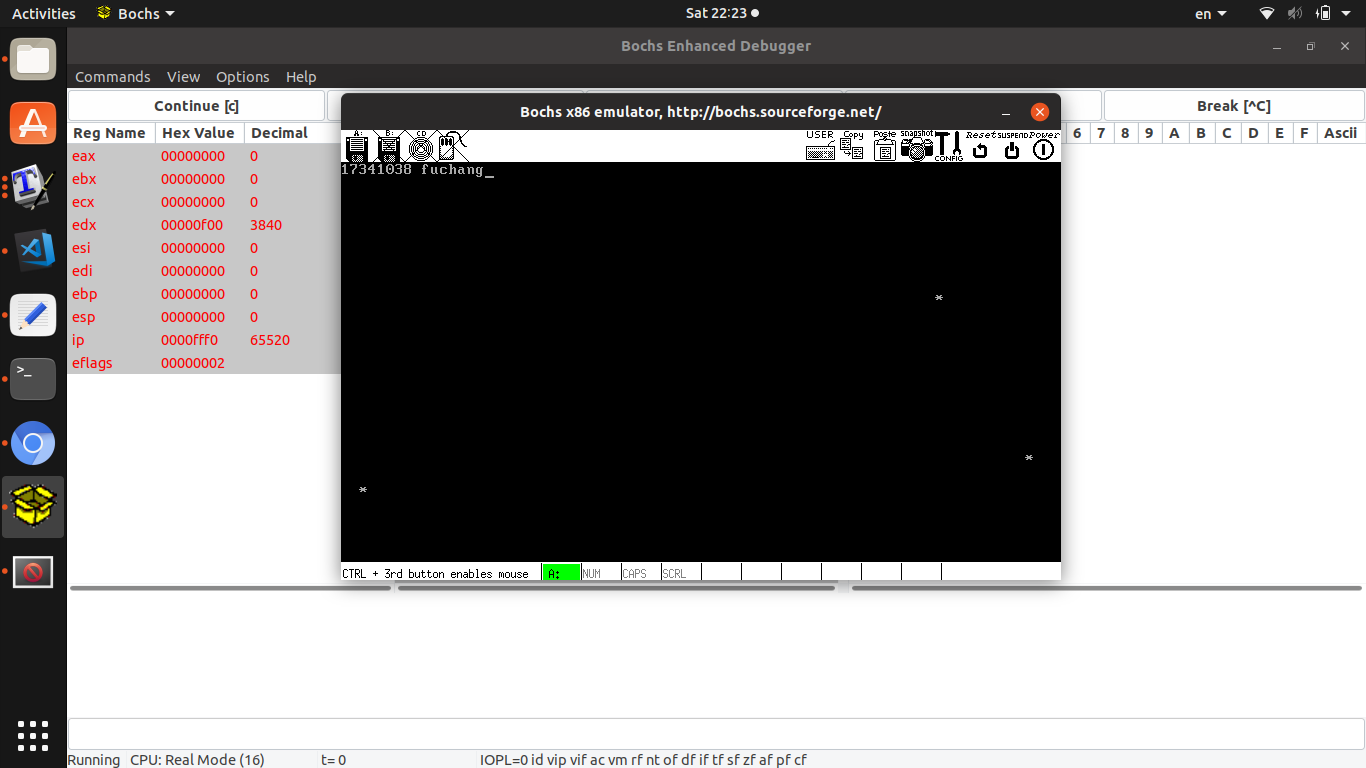
\includegraphics[width=10cm]{Screenshot from 2019-03-23 22-23-44.png}
		\bottomcaption{显示}
	\end{figure}


\subsection{疑难问题解决}
	
	\begin{itemize}
		\item nasm中乘除法的使用,很奇怪,它的默认被乘数/被除数是ax,部分商放在dl中
		
		\item 有的时候对存储单位长度不太敏感,进行寄存器寻址/内存寻址的时候市场忽略db, dw等长度的区别,导致计算偏移的时候引入很奇怪的bug
			
	\end{itemize}


\section{实验总结}

第一次写操作系统的实验,就向之前每学习一门语言总会以一个“Hello world”程序作为第一个程序;当我在课堂上第一次写出一个
mov byte,[es:0x00],“@”的时候,心情和以前接触一门新的语言一样,打开了一扇新的大门。
起步的程序并不难在算法,反而是学习编程的基本问题:怎样设计程序的逻辑,如何调试,特殊的语句用法如何尽快掌握。
而且操作系统的编程环境相比高级语言所配置的各种炫酷赏心悦目的界面,OS实验课要注定经历从无到有白手起家的感觉。这是OS相比学习其他项目更需要克服的一道心里障碍。
总之第一次实验给我的信心非常好。
\bibliographystyle{plain}
\bibliography{ref}

\clearpage



\end{document}
